% !TEX root = ../main.tex
\section{未知拓扑下的动力学与拓扑联合学习}

\subsection{动力学与结构联合辨识}

移除已知网络之后，模型必须同时回答两个彼此关联的问题：怎样的局部规律能够解释观测到的状态变化，哪些节点之间存在足以支持这种解释的连接。
直观上，
真正相互作用的节点应当在时间序列中留下稳定的条件依赖；
但由于状态变化具有随机性，
而且动力学学习器具有较强的函数逼近能力，
错误结构也可能被参数调整暂时掩盖。

本文把这种现象称为结构--动力学补偿。
例如，生成器给出过多邻居时，学习器可以减小单个邻居的平均作用，使总输入仍落在合理范围内。
这样得到的模型可能具有较低的一步损失，
却不能提供可信的连接解释。
未知网络任务因此不能只是“把邻接矩阵也设成参数”，
还需要限制结构与规律相互替代的自由度。

\subsection{可学习的离散拓扑}

本文为每个无序节点对维护一个可训练的连接倾向 $R_{ij}$，并通过 Gumbel--Softmax 和 Concrete 松弛产生可微的软邻接矩阵\cite{jang2017,maddison2017}：
\begin{equation}
\hat A_{ij}^{\mathrm{soft}}
=\sigma\!\left(\frac{R_{ij}+G_{ij}}{\tau}\right),
\qquad G_{ij}\sim\operatorname{Logistic}(0,1).
\label{eq:gumbel-soft}
\end{equation}
上三角变量被镜像到下三角，对角线固定为零，从而保证候选图无向且无自环。
需要输出具体网络时，使用 0.5 阈值得到硬连接
\begin{equation}
\hat A_{ij}^{\mathrm{hard}}=\mathbf{1}[R_{ij}+G_{ij}>0].
\label{eq:hard-sample}
\end{equation}
当连接倾向与采样噪声之和 $R_{ij}+G_{ij}>0$ 时，节点 $i$ 与 $j$ 之间保留一条边；
否则不保留该边。
温度 $\tau$ 改变软图的锐度与反向传播梯度，但在给定 $R_{ij}$ 和噪声时，并不直接改变 0.5 阈值下的硬采样结果。

生成的候选网络进入双通道动力学学习器。
自身通道仍描述节点内在变化，邻居通道则通过 $\hat A\,g(\mathbf X)$ 汇聚候选邻居的作用。
这样，
已知网络阶段形成的表示原则可以直接延伸到潜在网络：区别仅在于交互对象不再预先给出，
而要由观测数据共同确定。

\subsection{硬图规律学习与软图结构更新}

联合训练采用交替策略，如\cref{fig:joint-flow}所示。
在动力学学习阶段，从当前连接分布采样一张离散硬图，固定该图并更新双通道学习器。
由于每条边只能取 0 或 1，
学习器不能简单地把大量多余边都缩成很小的连续权重。
在结构更新阶段，
冻结学习器，
使用软图计算预测误差并把梯度传回连接倾向；
熵正则促使边概率远离难以解释的中间值。

\begin{figure}[H]
  \centering
  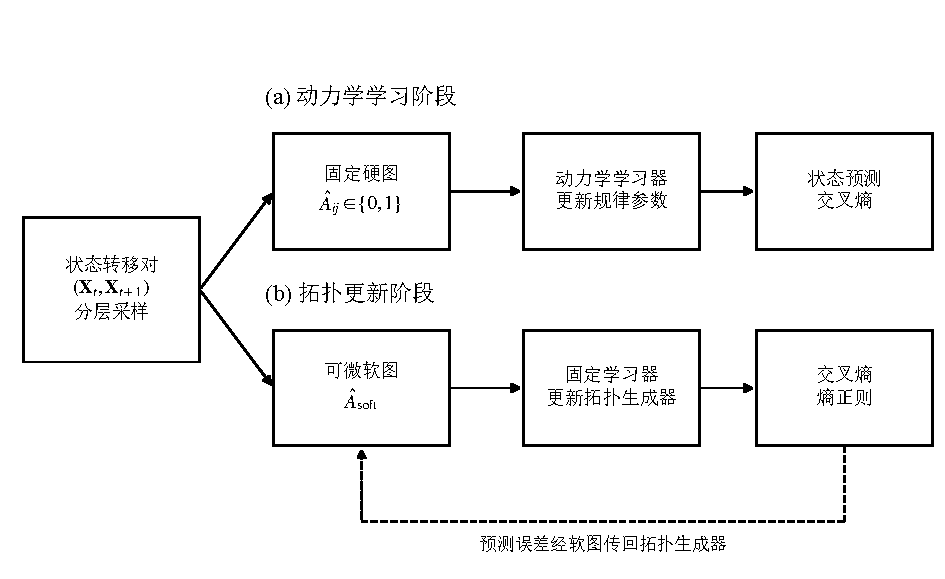
\includegraphics[width=\textwidth]{joint_training_flow.pdf}
  \caption{动力学与拓扑的交替学习。
硬图阶段更新演化规律，软图阶段利用可微松弛更新连接倾向；
两者共享同一预测目标，但承担不同的学习角色。}
  \label{fig:joint-flow}
\end{figure}

硬图学习削弱了连续弱边补偿。
本文进一步结合数据组织和模型选择，使连接辨识得到更充分的观测证据与验证信号。

\subsection{结构信息引导的分层采样}

传播轨迹中常有大量接近吸收态的时刻：系统中已经没有感染节点，或绝大多数节点只保持原状态。
这些样本有助于学习状态保持，却几乎不提供“影响沿哪条边传递”的信息。
如果训练始终被这类样本主导，
模型便可能在缺少结构证据的情况下优化出较低损失。

为此，本文按照每个时刻的感染节点数量分层，并在各层中无放回抽样，使低、中、高传播活动状态都能稳定进入每轮训练。
该设计在 SIR 中以感染者数量实现；
推广到其他动力学时，
可替换为状态变化幅度、活跃组分数量或局部事件强度等任务相关指标。
验证集仍保持原始分布，
避免选模只偏向重采样后的训练分布。

每类网络从三个不同初始化开始联合学习，最终只根据验证交叉熵选择一个模型，不使用真实边进行选模。
多初始化扩大了候选解的搜索范围，验证损失提供统一的选择依据。
完整的采样配额、训练节奏和九次运行结果均置于附录。
